% Options for packages loaded elsewhere
\PassOptionsToPackage{unicode}{hyperref}
\PassOptionsToPackage{hyphens}{url}
\PassOptionsToPackage{dvipsnames,svgnames*,x11names*}{xcolor}
%
\documentclass[
]{article}
\usepackage{amsmath,amssymb}
\usepackage{lmodern}
\usepackage{ifxetex,ifluatex}
\ifnum 0\ifxetex 1\fi\ifluatex 1\fi=0 % if pdftex
  \usepackage[T1]{fontenc}
  \usepackage[utf8]{inputenc}
  \usepackage{textcomp} % provide euro and other symbols
\else % if luatex or xetex
  \usepackage{unicode-math}
  \defaultfontfeatures{Scale=MatchLowercase}
  \defaultfontfeatures[\rmfamily]{Ligatures=TeX,Scale=1}
\fi
% Use upquote if available, for straight quotes in verbatim environments
\IfFileExists{upquote.sty}{\usepackage{upquote}}{}
\IfFileExists{microtype.sty}{% use microtype if available
  \usepackage[]{microtype}
  \UseMicrotypeSet[protrusion]{basicmath} % disable protrusion for tt fonts
}{}
\makeatletter
\@ifundefined{KOMAClassName}{% if non-KOMA class
  \IfFileExists{parskip.sty}{%
    \usepackage{parskip}
  }{% else
    \setlength{\parindent}{0pt}
    \setlength{\parskip}{6pt plus 2pt minus 1pt}}
}{% if KOMA class
  \KOMAoptions{parskip=half}}
\makeatother
\usepackage{xcolor}
\IfFileExists{xurl.sty}{\usepackage{xurl}}{} % add URL line breaks if available
\IfFileExists{bookmark.sty}{\usepackage{bookmark}}{\usepackage{hyperref}}
\hypersetup{
  colorlinks=true,
  linkcolor=blue,
  filecolor=Maroon,
  citecolor=Blue,
  urlcolor=blue,
  pdfcreator={LaTeX via pandoc}}
\urlstyle{same} % disable monospaced font for URLs
\usepackage[margin=1in]{geometry}
\usepackage{color}
\usepackage{fancyvrb}
\newcommand{\VerbBar}{|}
\newcommand{\VERB}{\Verb[commandchars=\\\{\}]}
\DefineVerbatimEnvironment{Highlighting}{Verbatim}{commandchars=\\\{\}}
% Add ',fontsize=\small' for more characters per line
\usepackage{framed}
\definecolor{shadecolor}{RGB}{248,248,248}
\newenvironment{Shaded}{\begin{snugshade}}{\end{snugshade}}
\newcommand{\AlertTok}[1]{\textcolor[rgb]{0.94,0.16,0.16}{#1}}
\newcommand{\AnnotationTok}[1]{\textcolor[rgb]{0.56,0.35,0.01}{\textbf{\textit{#1}}}}
\newcommand{\AttributeTok}[1]{\textcolor[rgb]{0.77,0.63,0.00}{#1}}
\newcommand{\BaseNTok}[1]{\textcolor[rgb]{0.00,0.00,0.81}{#1}}
\newcommand{\BuiltInTok}[1]{#1}
\newcommand{\CharTok}[1]{\textcolor[rgb]{0.31,0.60,0.02}{#1}}
\newcommand{\CommentTok}[1]{\textcolor[rgb]{0.56,0.35,0.01}{\textit{#1}}}
\newcommand{\CommentVarTok}[1]{\textcolor[rgb]{0.56,0.35,0.01}{\textbf{\textit{#1}}}}
\newcommand{\ConstantTok}[1]{\textcolor[rgb]{0.00,0.00,0.00}{#1}}
\newcommand{\ControlFlowTok}[1]{\textcolor[rgb]{0.13,0.29,0.53}{\textbf{#1}}}
\newcommand{\DataTypeTok}[1]{\textcolor[rgb]{0.13,0.29,0.53}{#1}}
\newcommand{\DecValTok}[1]{\textcolor[rgb]{0.00,0.00,0.81}{#1}}
\newcommand{\DocumentationTok}[1]{\textcolor[rgb]{0.56,0.35,0.01}{\textbf{\textit{#1}}}}
\newcommand{\ErrorTok}[1]{\textcolor[rgb]{0.64,0.00,0.00}{\textbf{#1}}}
\newcommand{\ExtensionTok}[1]{#1}
\newcommand{\FloatTok}[1]{\textcolor[rgb]{0.00,0.00,0.81}{#1}}
\newcommand{\FunctionTok}[1]{\textcolor[rgb]{0.00,0.00,0.00}{#1}}
\newcommand{\ImportTok}[1]{#1}
\newcommand{\InformationTok}[1]{\textcolor[rgb]{0.56,0.35,0.01}{\textbf{\textit{#1}}}}
\newcommand{\KeywordTok}[1]{\textcolor[rgb]{0.13,0.29,0.53}{\textbf{#1}}}
\newcommand{\NormalTok}[1]{#1}
\newcommand{\OperatorTok}[1]{\textcolor[rgb]{0.81,0.36,0.00}{\textbf{#1}}}
\newcommand{\OtherTok}[1]{\textcolor[rgb]{0.56,0.35,0.01}{#1}}
\newcommand{\PreprocessorTok}[1]{\textcolor[rgb]{0.56,0.35,0.01}{\textit{#1}}}
\newcommand{\RegionMarkerTok}[1]{#1}
\newcommand{\SpecialCharTok}[1]{\textcolor[rgb]{0.00,0.00,0.00}{#1}}
\newcommand{\SpecialStringTok}[1]{\textcolor[rgb]{0.31,0.60,0.02}{#1}}
\newcommand{\StringTok}[1]{\textcolor[rgb]{0.31,0.60,0.02}{#1}}
\newcommand{\VariableTok}[1]{\textcolor[rgb]{0.00,0.00,0.00}{#1}}
\newcommand{\VerbatimStringTok}[1]{\textcolor[rgb]{0.31,0.60,0.02}{#1}}
\newcommand{\WarningTok}[1]{\textcolor[rgb]{0.56,0.35,0.01}{\textbf{\textit{#1}}}}
\usepackage{longtable,booktabs,array}
\usepackage{calc} % for calculating minipage widths
% Correct order of tables after \paragraph or \subparagraph
\usepackage{etoolbox}
\makeatletter
\patchcmd\longtable{\par}{\if@noskipsec\mbox{}\fi\par}{}{}
\makeatother
% Allow footnotes in longtable head/foot
\IfFileExists{footnotehyper.sty}{\usepackage{footnotehyper}}{\usepackage{footnote}}
\makesavenoteenv{longtable}
\usepackage{graphicx}
\makeatletter
\def\maxwidth{\ifdim\Gin@nat@width>\linewidth\linewidth\else\Gin@nat@width\fi}
\def\maxheight{\ifdim\Gin@nat@height>\textheight\textheight\else\Gin@nat@height\fi}
\makeatother
% Scale images if necessary, so that they will not overflow the page
% margins by default, and it is still possible to overwrite the defaults
% using explicit options in \includegraphics[width, height, ...]{}
\setkeys{Gin}{width=\maxwidth,height=\maxheight,keepaspectratio}
% Set default figure placement to htbp
\makeatletter
\def\fps@figure{htbp}
\makeatother
% Make links footnotes instead of hotlinks:
\DeclareRobustCommand{\href}[2]{#2\footnote{\url{#1}}}
\setlength{\emergencystretch}{3em} % prevent overfull lines
\providecommand{\tightlist}{%
  \setlength{\itemsep}{0pt}\setlength{\parskip}{0pt}}
\setcounter{secnumdepth}{5}
\usepackage{booktabs}

% use cleverref package for cross references
% found at https://community.rstudio.com/t/bookdown-equations/38540 
\usepackage[noabbrev]{cleveref}
\renewcommand{\eqref}{\Cref}
\Crefformat{equation}{#2#1#3}
\usepackage{booktabs}
\usepackage{longtable}
\usepackage{array}
\usepackage{multirow}
\usepackage{wrapfig}
\usepackage{float}
\usepackage{colortbl}
\usepackage{pdflscape}
\usepackage{tabu}
\usepackage{threeparttable}
\usepackage{threeparttablex}
\usepackage[normalem]{ulem}
\usepackage{makecell}
\usepackage{xcolor}
\ifluatex
  \usepackage{selnolig}  % disable illegal ligatures
\fi
\newlength{\cslhangindent}
\setlength{\cslhangindent}{1.5em}
\newlength{\csllabelwidth}
\setlength{\csllabelwidth}{3em}
\newenvironment{CSLReferences}[2] % #1 hanging-ident, #2 entry spacing
 {% don't indent paragraphs
  \setlength{\parindent}{0pt}
  % turn on hanging indent if param 1 is 1
  \ifodd #1 \everypar{\setlength{\hangindent}{\cslhangindent}}\ignorespaces\fi
  % set entry spacing
  \ifnum #2 > 0
  \setlength{\parskip}{#2\baselineskip}
  \fi
 }%
 {}
\usepackage{calc}
\newcommand{\CSLBlock}[1]{#1\hfill\break}
\newcommand{\CSLLeftMargin}[1]{\parbox[t]{\csllabelwidth}{#1}}
\newcommand{\CSLRightInline}[1]{\parbox[t]{\linewidth - \csllabelwidth}{#1}\break}
\newcommand{\CSLIndent}[1]{\hspace{\cslhangindent}#1}

\author{}
\date{\vspace{-2.5em}}

\begin{document}

\hypertarget{analysis-tools}{%
\section{Analysis Tools}\label{analysis-tools}}

Data Analysis is inherently build upon two foundational components: High Quality Data that allows to gain insight into the underlying data generating process and a structured and reproducible way to extract information out of the collected data.

Thus, \Cref{data} introduces the two datasets we worked with whereas \Cref{package} provides an overview about the \texttt{postforecasts} package, a unified framework to apply and analyze various post-processing methods.

\hypertarget{data}{%
\subsection{Data \& Methodology}\label{data}}

This section first introduces the two data sources that all of our analysis is based on.
Afterwards, the final paragraphs explain our evaluation procedure from a theoretical view point.

\hypertarget{uk-covid-19-crowd-forecasting-challenge}{%
\subsubsection{UK Covid-19 Crowd Forecasting Challenge}\label{uk-covid-19-crowd-forecasting-challenge}}

As part of an ongoing research project by the \emph{epiforecasts} group at the London School of Hygiene \& Tropical Medicine the \href{https://www.crowdforecastr.org/2021/05/11/uk-challenge/}{UK Covid-19 Crowd Forecasting Challenge} consisted of submitting weekly predictions of Covid-19 Cases and Deaths in the United Kingdom.
The challenge was not restricted to experienced researchers in the field but rather intended to collect quantile predictions for the upcomning four weeky by non-expert individuals.

One of the main motivations was to gather evidence for or against the hypotheses that humans are highly capable of submitting precise \emph{point forecasts}, yet, at the same time, they tend to be too confident in their beliefs such that prediction \emph{intervals} are chosen too narrow.
In fact, this tendency represents one motivation for post-processing: Extract valuable information from point forecasts and adjust the corresponding prediction intervals with a systematic correction procedure.

In case of individuals that are unfamiliar with statistical methodology specifying forecasts for \(23\) quantiles ranging from 0.01 to 0.99 separately might lead to inconsistencies.
Therefore all participants could determine an uncertainty parameter around their median prediction via an interactive web application such that all quantile predictions could be concluded in an automatic fashion.
Note that this procedure leads to \emph{symmetric} forecast intervals.

The results of the 12-week challenge are \href{https://epiforecasts.io/uk-challenge/}{publicly available}.

\hypertarget{european-covid-19-forecast-hub}{%
\subsubsection{European Covid-19 Forecast Hub}\label{european-covid-19-forecast-hub}}

According to their \href{https://covid19forecasthub.eu/index.html}{webpage} the European Covid-19 Forecast Hub collects \emph{short-term forecasts of Covid-19 cases and deaths across Europe, created by a multitude of infectious disease modelling teams}.

In contrast to the compact UK data described above, the European Forecast Hub data contains almost two million observations for over \(20\) European countries.
Further, the forecasters are knowledgeable research groups that submit their weekly predictions based on statistical models.
Although the data collection continues in regular frequency up to this day, our data set is limited to a \(32\)-week span from March \(2021\) until October \(2021\).

\hypertarget{weighted-interval-score}{%
\subsubsection{Weighted Interval Score}\label{weighted-interval-score}}

In order to quantify if the post-processed prediction intervals improve the original forecasts we chose the \emph{Weighted Interval Score} (WIS) (Bracher et al. 2021) as our evaluation metric.
The WIS is a so-called \emph{Proper Scoring Rule} (Gneiting and Raftery 2007): It incentivizes the forecaster to state their true best belief and cannot be manipulated to its own benefit.
It combines measures for interval \emph{sharpness} as well as \emph{overprediction} and \emph{underprediction} and can thus be understood as a trade-off between prediction \emph{accuracy} and \emph{precision}.

More specifically, for a given quantile level \(\alpha\), true observed value \(y\) as well as lower bound \(l\) and upper bound \(u\) of the corresponding \((1 - \alpha) \cdot 100\)\% prediction interval, the Weighted Interval Score is computed as
\[
\begin{equation}
Score_\alpha(y) 
= (u-l) + \frac{2}{\alpha} \cdot (l-y) \cdot \mathbf{1} (y \leq l) + \frac{2}{\alpha} \cdot (y-u) \cdot \mathbf{1}(y \geq u).
\label{eq:binom}
\end{equation}
\]
The score of an entire model can then be obtained from a weighted sum over all (included) quantile levels \(\alpha\).

\hypertarget{time-series-cross-validation}{%
\subsubsection{Time Series Cross Validation}\label{time-series-cross-validation}}

Just like any statistical model the post-processing methods must be evaluated on \emph{out-of-sample} data.
Rather than starting from the raw data, i.e.~the observed Covid-19 Cases and Deaths, our data sets already consist of existing quantile predictions.
As a consequence, no part of our data set must be dedicated to fitting the quantile regression models in the first place and our evaluation procedure can be split in two steps:

\begin{enumerate}
\def\labelenumi{\arabic{enumi}.}
\item
  Use a \emph{training set} to learn parameters of the post-processing procedure in consideration.
\item
  Use a \emph{validation set} to evaluate how the learned parameters generalize to unseen data.
\end{enumerate}

Instead of a hard cut-off between the splits we used \emph{Time Series Cross Validation} to leverage a higher fraction of the data set for training.
In contrast to classical cross validation for independent and identically distributed data, time series cross validation iterates through the data set along the time dimension one step at a time.

The process is nicely illustrated in \Cref{fig:ch1-cv}\footnote{Image Source: \url{https://otexts.com/fpp3/tscv.html} (Hyndman and Athanasopoulos 2021).}.

\begin{figure}

{\centering 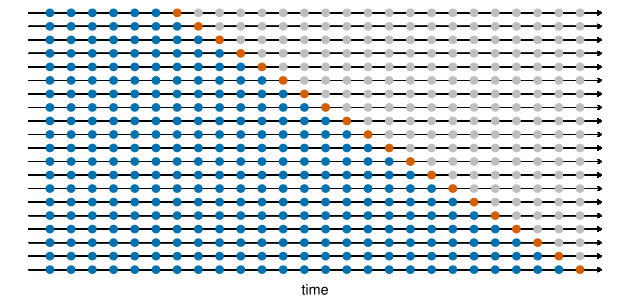
\includegraphics[width=0.8\linewidth]{/Users/maherp/Desktop/Universitaet/Goettingen/3_Semester/Statistisches_Praktikum/post-processing-forecasts/term_paper/images/cv-hyndman} 

}

\caption{Time Series Cross Validation}\label{fig:ch1-cv}
\end{figure}

At each iteration the validation set is composed of the one step ahead prediction based on all observations prior to and including the current time point.
The algorithm typically starts with a minimum number of observations as the initial training set, which can be considered a hyperparameter that has to be specified at the beginning of training.

\hypertarget{package}{%
\subsection{\texorpdfstring{The \texttt{postforecasts} Package}{The postforecasts Package}}\label{package}}

One core aspect of our project was the development of a fully functional R package that unites a collection of different post-processing algorithms into a well-designed and user friendly interface.
This section can be understood as a compact guide how to use our package effectively and explains some of the thought process that went into the implementation.
It is worth noting that the \texttt{postforecasts} package adheres to all formal requirements for an R package such that \texttt{RCMDCHECK} does not produce any warnings or errors.

\hypertarget{overview}{%
\subsubsection{Overview}\label{overview}}

The \texttt{postforecasts} functions that are meant to be visible to the end-user can be grouped into three categories:

\begin{enumerate}
\def\labelenumi{\arabic{enumi}.}
\item
  Exploratory

  The \texttt{plot\_quantiles()}, \texttt{plot\_intervals()} and \texttt{plot\_intervals\_grid()} functions visualize the development of true Covid19 Cases and Deaths over time as well as corresponding original and post-processed quantile predictions.
\item
  Model Fitting

  The \texttt{update\_predictions()} function is the workhorse of the entire \texttt{postforecasts} package.
  It specifies both the raw data and the post-processing method(s) that should be applied to this data set.
  The function returns a list of \(k+1\) equally shaped data frames for \(k\) selected post-processing methods, the first element being the original, possibly filtered, data frame.

  All list elements can be analyzed separately or collectively by stacking them into one large data frame with the \texttt{collect\_predictions()} function.
  The combined data frame is designed to work well with analysis functions that are provided by the \href{https://epiforecasts.io/scoringutils/}{scoringutils package} (Bosse, Sam Abbott, and Gruson 2022).
  Finally, an ensemble model of all selected methods can be appended which will be explained in \Cref{comparison} .
\item
  Evaluation

  As noted in \Cref{data} the Weighted Interval Score is our primary metric to evaluate the \emph{quality} of prediction intervals.
  The \texttt{score()} function of the \texttt{scoringutils} package computes this score for each observation in the data set which can then be aggregated by the related \texttt{summarise\_scores()} function.
  Depending on the \emph{granularity} of the aggregation the output might contain many interval scores of vastly different magnitudes.
  To simplify interpretation the \texttt{eval\_methods()} function computes \emph{relative} or \emph{percentage} changes in the Weighted Interval Score for each selected method compared to the original quantile predictions.
  Further, these relative changes can be conveniently visualized by the \texttt{plot\_eval()} function.
\end{enumerate}

The following section demonstrates the complete workflow described above to give an impression how all these functions interact.

\hypertarget{workflow}{%
\subsubsection{Workflow}\label{workflow}}

We use the Covid-19 data for Germany in \(2021\) that is provided by the European Forecast Hub.

\Cref{fig:ch1-quantiles-germany} illustrates the \(5\)\%, \(20\)\% \(80\)\% and \(95\)\% quantile predictions of the \texttt{EuroCOVIDhub-ensemble} during the summer months of \(2021\) in Germany.

\begin{Shaded}
\begin{Highlighting}[]
\FunctionTok{plot\_quantiles}\NormalTok{(}
\NormalTok{  hub\_germany,}
  \AttributeTok{model =} \StringTok{"EuroCOVIDhub{-}ensemble"}\NormalTok{, }\AttributeTok{quantiles =} \FunctionTok{c}\NormalTok{(}\FloatTok{0.05}\NormalTok{, }\FloatTok{0.2}\NormalTok{, }\FloatTok{0.8}\NormalTok{, }\FloatTok{0.95}\NormalTok{)}
\NormalTok{)}
\end{Highlighting}
\end{Shaded}

\begin{figure}

{\centering \includegraphics[width=1\linewidth]{1_data_package_files/figure-latex/ch1-quantiles-germany-1} 

}

\caption{Original Quantile Predictions for Covid-19 Cases and Deaths in Germany 2021}\label{fig:ch1-quantiles-germany}
\end{figure}

The original predictions look quite noisy overall with the clear trend that uncertainty and the interval width increases with growing forecast horizon.
Thus, we want to analyze if one particular post-processing method, \emph{Conformalized Quantile Regression} which is explained in much more detail in \Cref{cqr}, improves the predictive performance for this model on a validation set by computing the Weighted Interval Scores for Covid Cases and Covid Deaths separately.

\begin{Shaded}
\begin{Highlighting}[]
\NormalTok{df\_updated }\OtherTok{\textless{}{-}} \FunctionTok{update\_predictions}\NormalTok{(}
\NormalTok{  hub\_germany,}
  \AttributeTok{methods =} \StringTok{"cqr"}\NormalTok{, }\AttributeTok{models =} \StringTok{"EuroCOVIDhub{-}ensemble"}\NormalTok{, }\AttributeTok{cv\_init\_training =} \FloatTok{0.5}
\NormalTok{)}
\NormalTok{df\_combined }\OtherTok{\textless{}{-}} \FunctionTok{collect\_predictions}\NormalTok{(df\_updated)}
\end{Highlighting}
\end{Shaded}

\begin{Shaded}
\begin{Highlighting}[]
\NormalTok{df\_combined }\SpecialCharTok{|}\ErrorTok{\textgreater{}}
  \FunctionTok{extract\_validation\_set}\NormalTok{() }\SpecialCharTok{|}\ErrorTok{\textgreater{}}
\NormalTok{  scoringutils}\SpecialCharTok{::}\FunctionTok{score}\NormalTok{() }\SpecialCharTok{|}\ErrorTok{\textgreater{}}
\NormalTok{  scoringutils}\SpecialCharTok{::}\FunctionTok{summarise\_scores}\NormalTok{(}\AttributeTok{by =} \FunctionTok{c}\NormalTok{(}\StringTok{"method"}\NormalTok{, }\StringTok{"target\_type"}\NormalTok{))}
\end{Highlighting}
\end{Shaded}

\begin{table}

\caption{\label{tab:ch1-wis-table}Comparison of the Weighted Interval Score after CQR Adjustments}
\centering
\begin{tabular}[t]{cccc}
\toprule
method & target\_type & interval\_score & dispersion\\
\midrule
cqr & Cases & 13.37 & 5.05\\
original & Cases & 13.78 & 3.81\\
cqr & Deaths & 0.05 & 0.01\\
original & Deaths & 0.05 & 0.03\\
\bottomrule
\end{tabular}
\end{table}

\Cref{tab:ch1-wis-table} shows that CQR improved the Weighted Interval Score for Covid Cases on the validation set, whereas the predictive performance for Covid Deaths dropped slightly.

The \texttt{update\_predictions()} and \texttt{collect\_predictions()} combination immediately generalize to multiple post-processing methods.
The only syntax change is a vector input of strings for the \texttt{methods} argument instead of a single string.
Hence, if not desired, the user does not have to worry about which input and output features each method requires in its raw form nor how exactly each method is implemented.
This design allows for maximum syntactic consistency through masking internal functionality.

In the output above CQR increased the \emph{dispersion} of the predictions for Cases significantly.
These wider intervals for specific covariate combinations are visualized in \Cref{fig:ch1-intervals-germany}.

\begin{Shaded}
\begin{Highlighting}[]
\FunctionTok{plot\_intervals}\NormalTok{(df\_combined, }\AttributeTok{target\_type =} \StringTok{"Cases"}\NormalTok{, }\AttributeTok{horizon =} \DecValTok{2}\NormalTok{, }\AttributeTok{quantile =} \FloatTok{0.05}\NormalTok{)}
\end{Highlighting}
\end{Shaded}

\begin{figure}

{\centering \includegraphics[width=1\linewidth]{1_data_package_files/figure-latex/ch1-intervals-germany-1} 

}

\caption{Original and CQR-adjusted Prediction Intervals for Covid-19 Cases in Germany}\label{fig:ch1-intervals-germany}
\end{figure}

Indeed, the 2 weeks-ahead \(90\)\% prediction intervals for Cases in Germany are increased by CQR.
The grey dashed line indicates the end of the training set within the time-series cross validation process.

Recall that uncertainty increases with larger horizons.
Similarly, CQR adjustments also increase in size for forecasts that are submitted further in advance, which can be seen in \Cref{fig:ch1-intervalsgrid-germany}.

\begin{Shaded}
\begin{Highlighting}[]
\FunctionTok{plot\_intervals\_grid}\NormalTok{(df\_combined, }\AttributeTok{facet\_by =} \StringTok{"horizon"}\NormalTok{, }\AttributeTok{quantiles =} \FloatTok{0.05}\NormalTok{)}
\end{Highlighting}
\end{Shaded}

\begin{figure}

{\centering \includegraphics[width=1\linewidth]{1_data_package_files/figure-latex/ch1-intervalsgrid-germany-1} 

}

\caption{Original and CQR-adjusted Prediction Intervals for different Forecast Horizons}\label{fig:ch1-intervalsgrid-germany}
\end{figure}

Interestingly, CQR expands the intervals only for Cases whereas the forecasts for Deaths are narrowed!

Besides the target type (Cases or Deaths), it is also useful to compare CQR effects across forecast horizons or quantiles.
Quite intuitively, CQR generally has a stronger \emph{relative} benefit for large time horizons and extreme quantiles, where the original forecaster faced a greater uncertainty.
\Cref{fig:ch1-eval-germany} illustrates how, in special cases like this one, the effect on the validation set can show rather mixed trends due to disadvantageous adjustments for the two and three weeks-ahead \(98\)\% prediction intervals.

\begin{Shaded}
\begin{Highlighting}[]
\NormalTok{df\_eval }\OtherTok{\textless{}{-}} \FunctionTok{eval\_methods}\NormalTok{(df\_combined, }\AttributeTok{summarise\_by =} \FunctionTok{c}\NormalTok{(}\StringTok{"quantile"}\NormalTok{, }\StringTok{"horizon"}\NormalTok{))}
\FunctionTok{plot\_eval}\NormalTok{(df\_eval)}
\end{Highlighting}
\end{Shaded}

\begin{figure}

{\centering \includegraphics[width=1\linewidth]{1_data_package_files/figure-latex/ch1-eval-germany-1} 

}

\caption{Relative Changes in the WIS through CQR for all Quantile-Horizon combinations}\label{fig:ch1-eval-germany}
\end{figure}

\hypertarget{refs}{}
\begin{CSLReferences}{1}{0}
\leavevmode\hypertarget{ref-R-scoringutils}{}%
Bosse, Nikos, Sam Abbott, and Hugo Gruson. 2022. \emph{Scoringutils: Utilities for Scoring and Assessing Predictions}.

\leavevmode\hypertarget{ref-bracher2021}{}%
Bracher, Johannes, Evan L. Ray, Tilmann Gneiting, and Nicholas G. Reich. 2021. {``Evaluating Epidemic Forecasts in an Interval Format.''} \emph{PLOS Computational Biology} 17 (2): e1008618. \url{https://doi.org/10.1371/journal.pcbi.1008618}.

\leavevmode\hypertarget{ref-gneiting2007}{}%
Gneiting, Tilmann, and Adrian E Raftery. 2007. {``Strictly {Proper Scoring Rules}, {Prediction}, and {Estimation}.''} \emph{Journal of the American Statistical Association} 102 (477): 359--78. \url{https://doi.org/10.1198/016214506000001437}.

\leavevmode\hypertarget{ref-hyndman2021}{}%
Hyndman, Rob, and George Athanasopoulos. 2021. \emph{Forecasting: Principles and Practice}. Third. {OTexts}. \url{https://otexts.com/fpp3/}.

\end{CSLReferences}

\end{document}
